\documentclass{article}
\usepackage[a4paper,top=3.5cm,bottom=5cm,left=3.8cm,right=3.8cm,marginparwidth=1.75cm]{geometry}
\usepackage{graphicx} % Required for inserting images
\usepackage{float}
\usepackage{hyperref}

\usepackage{cite}

\title{\textbf{Intent Extraction\\ for Catalan Smart Home Commands}\\\textit{Porject Report}\\\Large{Natural Language Processing}}
\author{Ricard Renalias \and Eric Roy}
\date{April 2025}

\begin{document}

\maketitle
% Should we comment this?
\tableofcontents
\newpage

\section{Introduction}

HomeAssistant \cite{homeassistant} is an open-source software framework used to automate home devices. It focuses on local control (i.e. self-hosted) and in privacy.
One of the latest features of HomeAssistant is the ability to control the devices using your voice, using the pipeline schematized in figure \ref{fig:ha-pipeline}.

\begin{figure}[H]
    \centering
    \includegraphics[width=0.75\linewidth]{pipeline_home_assistant.png}
    \caption{
    HomeAssistant's voice command's pipeline (extracted from \cite{homeassistantvoice}).
    The user connects itself to the Assist Pipeline, which will be the process handling all
    the steps. It first converts the speech to text (STT), then it uses \textit{Conversation} to
    execute the actions and get a text response, and finally, if a response is needed, it
    converts the output text to speech (TTS). This enables the possibility to still talking directly with text without changing the entire system (by removing steps 2, 3, 8 and 9.
    }
    \label{fig:ha-pipeline}
\end{figure}

This system works very well with English, but some languages (like Catalan) have a lot of variations (for example: conjugations or sentence orders) which makes word scanning more complex. Moreover, inverted sentences (for example, sentences that start with 'No') might not be correctly detected. There are some solutions to this problem, but the ones supporting the Catalan language are very poor.

\begin{figure}[H]
    \centering
    \includegraphics[width=0.8\linewidth]{drawing2.png}
    \caption{
    Our simplification of the \textit{Conversation} module used to develop this project. Once we verify that it works correctly with this environment (that's easier to test) we will be able to easily use it in the real scenario.
    }
    \label{fig:our-pipeline-real}
\end{figure}

\subsection{Objective}

This project aims to set up a working system of HomeAssistant (as in figure \ref{fig:ha-pipeline}) to enable voice control in Catalan. We will use already existing parts for everyting except for the \textit{Conversation} module. The goal of this project is to replace this text scanning module with our own, more robust module. The module will have an architecture similar to figure \ref{fig:our-pipeline-real}.

\subsection{Related work}

Our work is based on OpenAI's whisper \cite{whisper} and BERT \cite{Moradi2019survey}. As stated in the project proposal, we will also be using HomeAssistant's data \cite{homeassistant} to have a dataset to start with.

However, while doing the project we also discoered project Aina \cite{hernandezmena2024_3catparla}, which contains many hours of catalan voices. We planned to use Whisper already, but we wanted to mention this project. Also, we were informed about the existence of SetFix \cite{tunstall2022efficient} which is a transformer that can be
trained with few samples. We nevertheless sticked to the original plan of fine-tunint BERT.

\section{Dataset preparation}

To fine-tune the model we will need a dataset relating sentences and actions. We will generate the dataset ourselves (and with the help of generative tools), since fine-tuning a model does not require a lot of data. The UPC has GPU servers available to the students that we can use to train it, but we suspect it won't be that much necessary.

HomeAssistant ecosystem community created a git repository \cite{homeassistant_intents} to generate all the intents requests from text in different languages.
For each language a set of typical text sentence instructions has been defined to allow working with assist.
In our case, we are interested to expand those yaml files in a format that can be used to train our BERT model. 

We have generated a Jupyter notebook that expands all the possible phrases to generate each intent. The output is saved in a \textit{jsonl} file to be able to use it in next steps.

\begin{itemize}
    \item Copy the Catalan language YAML files into the repository and prune the ones that are not useful or badly formatted.
    \item Execute the notebook to expand all the possible sentences for each intent.
    \item Review the generated output.
\end{itemize}

After a few iterations we end up with $25000$ rows of sentences to turn on and off devices.

\subsection{Intent expansion}

The main purpose of the Jupyter notebook is to convert a HomeAssistant regex of this
form:

\begin{verbatim}
engega|encen el {device} del|(de la) {area}
\end{verbatim}

To multiple samples by using all possible permutations. In the following text
we replaced \textit{device} for \textit{llum} and \textit{area} for \textit{labavo}. However, we use multiple values for these fields. You can easily see how fast this can grow.

\begin{verbatim}
engega el llum del lavabo
encen el llum de la lavabo
engega el llum de la lavabo
encen el llum del lavabo
\end{verbatim}

The hardest part, though, is to map each part of the sentence with a label. It's straight forward to map the devices and areas to a label, but we have used a bit of code to map the action.

\begin{figure}[H]
    \centering
    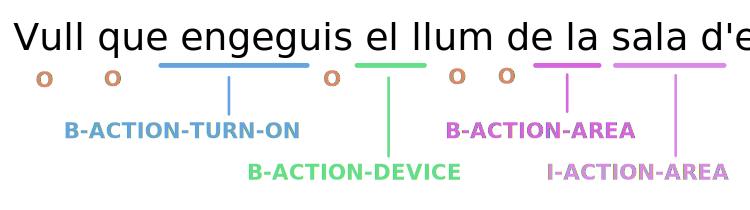
\includegraphics[width=0.75\linewidth]{bio_example.png}
    \caption{We do BIO labelling on our sentences to train afterwards. We tag with \textit{O} the words that are not useful, with \textit{B-Tag} the words that belong to a tag, and with \textit{I-Tag} words that belong to a tag but are the continuation to the previous one. This is needed in order to make sure that, in the example, \textit{sala d'estar} is an area and not two concatenated places.}
    \label{fig:bio-example}
\end{figure}

We end up in a jsonl file that relates the sentences with their labels, that will be used in the next section to train the model.

\subsection{LLM data}

We complimented the previous data with some generated by the help of the most recent ChatGPT model. The prompt was straight-forward: \textit{Generate 50 items with the format as the above jsonl example. Include formulations like "Pordies si us plau engegar ..."}. Using multiple formulations we obtained over a hundred of samples.

Then these samples are passed through a script that expands them, creating some misspellings, and concatenated with the previous dataset.

\section{Training}

We finally decided to train a BERT model for this project. We first did some tests with a BERT classifier, but seeing the poor results we decided to switch to something more sophisticated, like a NER.

\subsection{Named Entity Recognition}

As demonstrated in figure \ref{fig:bio-example}, there are only some parts of the sentence that are important to us. If we can train BERT to only pay attention to those parts (if present), we can even retrieve the name of the room (thus having infinite room names, compared to a classifier, that would require to re-train the model).

Thankfully, the \verb|transformers| python module is prepared for NER training, which made the progress very straightforward. Due to our hardware limitations, we trained with a batch of 70 samples at a time, since more made our system crash. We believe that a higher batch size would result in a better model.

With only 5 epochs we can see that the loss is reduced a lot, and by testing the model with the validation split (we did an 80-20 split) we can ensure ourselves that we aren't overfitting.

\section{Inferring}

This section details the taken steps to test the model in a somewhat-real environment.

\subsection{Speech-To-Text}

As said in the introduction, we used Whisper to convert the speech to text. We used typical Python packages to record the voice and prepare it for OpenAI's model. This process was straightforward and required few tuning.

As stated in \cite{whisper}, there are many provided models, some of which only for english. We tried different multilingual models and we decided to stay with the \textit{turbo} model, that has very good performance for only a few gigabytes of RAM.

\subsection{Model inferring}

Once the text is provided, we can pass it to our model. For this, we use the same system as for the training (when validating) to find the labels found, and we return to the user the list of labels found and their attached text. From this list we can easily convert it to HomeAssistant commands.

We finally didn't use the HomeAssistant API due to time restrictions, but it will be a nice addition to this project.

\section{Results}

The results of the previous model are pretty consistent when trained with many epochs.
Below are some examples. Note that there are some typos and the model is prepared for them.

\begin{verbatim}
Input: Pos obrir les persianes si us plau?
{'action-turn-on': 'obrir', 'device': 'persianes'}

Input: M'agradaria apagar el llum del safareig.
{'action-turn-off': 'apagar', 'device': 'llum', 'location': 'safareig.'}

Input: Paga la radio
{'device': 'radio'}
\end{verbatim}

We're pretty pleased with these results, since these sentences differ strongly from the dataset (in purpose), and the model still outputs good results. On the last example it is a shame that the model didn't understand \textit{Paga} as a misspelling of \textit{Apaga}, but this could be easily fixed by adding some cases like this in the training dataset.

\section{Conclusions}

In this project we've been able to play with natural language processing tools such as Speech-To-Text tools, Named Entity Recognition, Transformers, and all of this within open-source software. Although we didn't reach all the planned goals, we submitted a functional system that demonstrates that the transformer can be trained with a very short dataset and provide very accurate results.

A great extension to this work would be to integrate it into HomeAssistant, but also to replace the model with an LLM and discover how better or worse the latter performs compared to our work.
Figure \ref{fig:utopic} exposes an architecture improvement if we still wan to fine-tune models.

\begin{figure}
    \centering
    \includegraphics[width=0.9\linewidth]{utopic.png}
    \caption{A better architecture (and more sophisticated) would be one that extracts separately (using NER or classifiers depending on the case) the information from the sentence. Classifiers could be combined if necessary to spare some resources.}
    \label{fig:utopic}
\end{figure}

% \bibliographystyle{apalike}
\bibliographystyle{plain}
\bibliography{mybib}

\end{document}
